\begin{table}
    \centering
    \caption{Beim Kurzschließen des $50\Omega$-Kables gemessene Werte für $R_{50},C_{50},L_{50}$ und daruas berechnete Werte für $G_{50}$ bei den jeweils eingestellten Frequenzen $f$}
    \label{tab:RLC50Werte}
    \sisetup{parse-numbers=false}
    \begin{tabular}{
	S[table-format=3.1]
	S[table-format=1.4]
	S[table-format=3.1]
	S[table-format=1.2]
	S[table-format=1.1]
	}
	\toprule
	{$f_{50} \ \mathrm{in} \ \si{\kilo\hertz}$}		& {$R_{50} \ \mathrm{in} \ \si{\ohm}$}		& 
	{$C_{50} \ \mathrm{in} \ \si{\pico\farad}$}		& {$L_{50} \ \mathrm{in} \ \si{\micro\henry}$}		& 
	{$G_{50} \ \mathrm{in} \ \si{\milli\siemens}$}		\\ 
	\midrule
    100.0 & 0.6402 & 987.4 & 3.12 & 0.2 \\
20.0  & 0.5572 & 986.6 & 3.18 & 0.2 \\
18.0  & 0.5556 & 986.6 & 3.18 & 0.2 \\
16.0  & 0.5546 & 986.6 & 3.18 & 0.2 \\
14.0  & 0.5537 & 986.5 & 3.18 & 0.2 \\
12.0  & 0.5530 & 986.5 & 3.18 & 0.2 \\
10.0  & 0.5523 & 986.5 & 3.18 & 0.2 \\
8.0   & 0.5518 & 986.5 & 3.19 & 0.2 \\
6.0   & 0.5513 & 986.5 & 3.19 & 0.2 \\
4.0   & 0.5510 & 986.5 & 3.19 & 0.2 \\
3.0   & 0.5508 & 986.5 & 3.19 & 0.2 \\
2.0   & 0.5506 & 986.5 & 3.18 & 0.2 \\
1.0   & 0.5506 & 986.7 & 3.20 & 0.2 \\
0.8   & 0.5506 & 986.7 & 3.10 & 0.2 \\
0.6   & 0.5505 & 986.7 & 3.10 & 0.2 \\
0.6   & 0.5504 & 986.7 & 3.00 & 0.2 \\
0.2   & 0.5505 & 986.7 & 2.20 & 0.2 \\

    \bottomrule
    \end{tabular}
    \end{table}

\begin{table}
    \centering
    \caption{Beim Kurzschließen des $75\Omega$-Kables gemessene Werte für $R_{75},C_{75},L_{75}$ und daraus berechnete Werte für $G_{75}$ bei den jeweils eingestellten Frequenzen $f$}
    \label{tab:RLC75Werte}
    \sisetup{parse-numbers=false}
    \begin{tabular}{
	S[table-format=3.0]
	S[table-format=1.2]
	S[table-format=3.1]
	S[table-format=1.2]
	S[table-format=1.1]
	}
	\toprule
	{$f_{75} \ \mathrm{in} \ \si{\kilo\hertz}$}		& {$R_{75} \ \mathrm{in} \ \si{\ohm}$}		& 
	{$C_{75} \ \mathrm{in} \ \si{\pico\farad}$}		& {$L_{75} \ \mathrm{in} \ \si{\micro\henry}$}		& 
	{$G_{75} \ \mathrm{in} \ \si{\milli\siemens}$}		\\ 
	\midrule
    100 & 6.90 & 672.5 & 4.28 & 1.1 \\
20  & 6.40 & 671.8 & 5.30 & 0.8 \\
18  & 6.35 & 671.8 & 5.40 & 0.8 \\
16  & 6.30 & 671.7 & 5.51 & 0.8 \\
14  & 6.24 & 671.7 & 5.63 & 0.7 \\
12  & 6.23 & 671.7 & 5.78 & 0.7 \\
10  & 6.11 & 671.7 & 5.91 & 0.7 \\
8   & 6.06 & 671.7 & 6.06 & 0.7 \\

    \bottomrule
    \end{tabular}
    \end{table}

\begin{figure}[h]
	\centering
	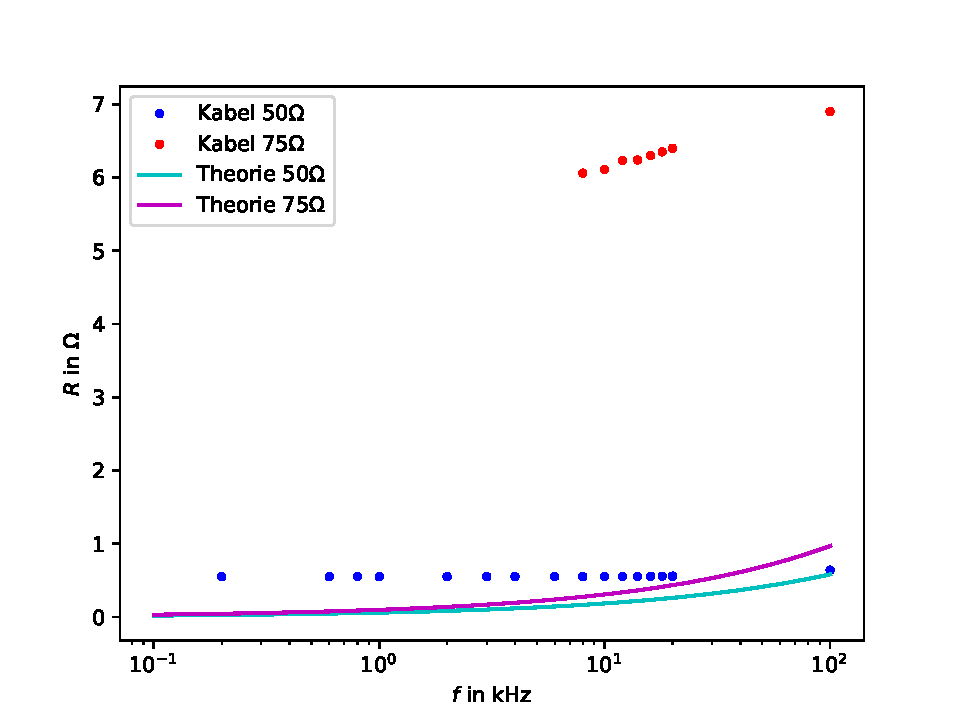
\includegraphics[width=0.8\textwidth]{RLC_DirekteMessung/build/PlotR.pdf}
	\caption{Gemessene Werte für $R$ beim Kurzschluss mit Theoriewert}
	\label{fig:PlotR}
\end{figure}
\begin{figure}[h]
	\centering
	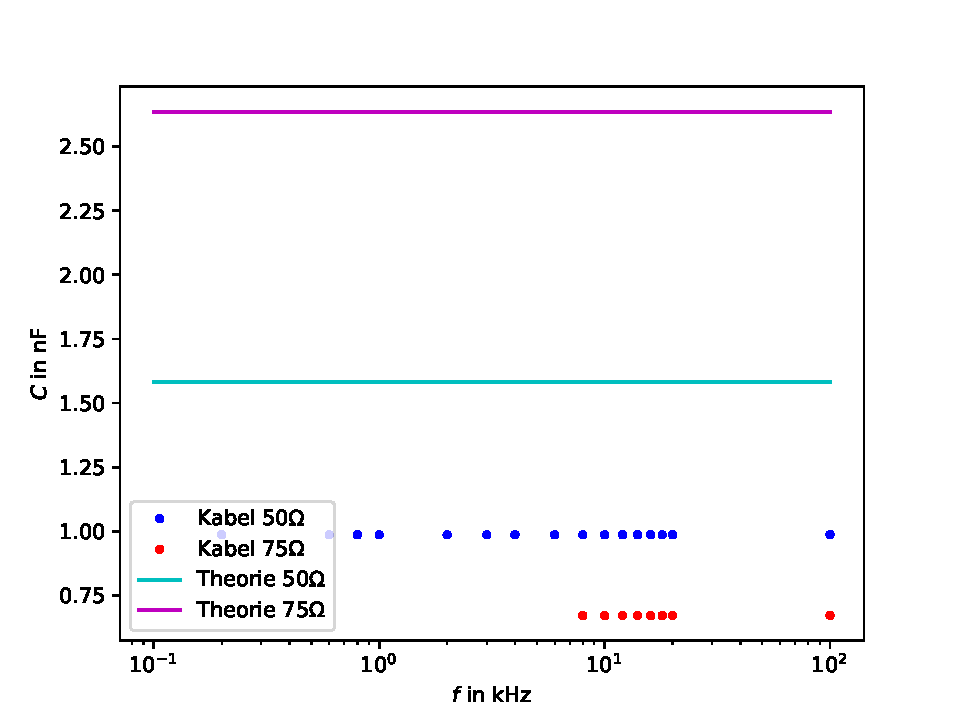
\includegraphics[width=0.8\textwidth]{RLC_DirekteMessung/build/PlotC.pdf}
	\caption{Gemessene Werte für $C$ beim Kurzschluss mit Theoriewert}
	\label{fig:PlotC}
\end{figure}
\begin{figure}[h]
	\centering
	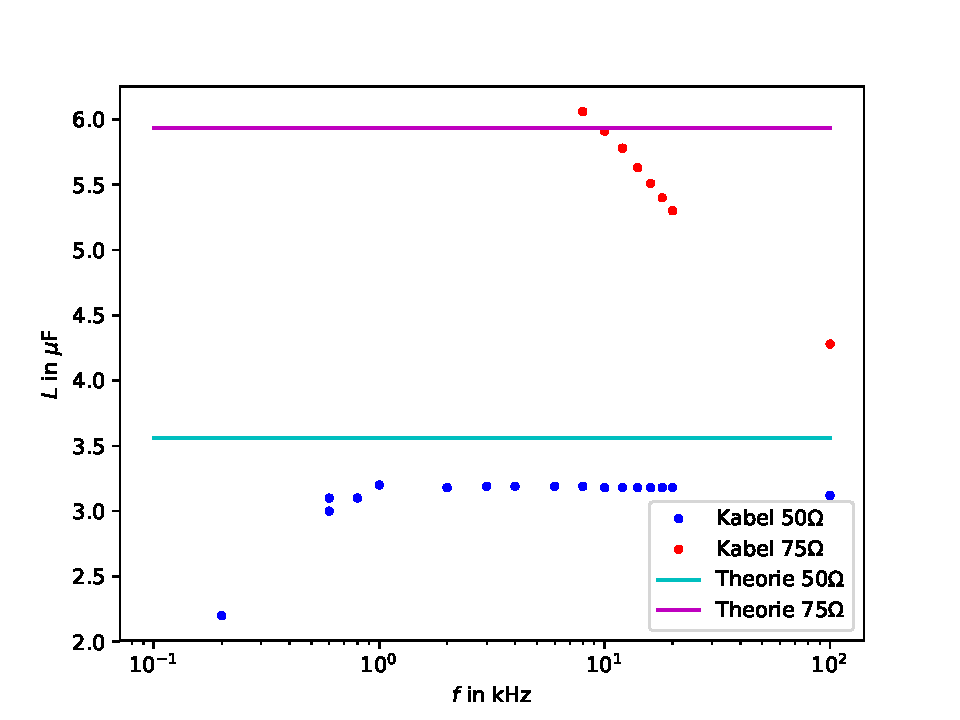
\includegraphics[width=0.8\textwidth]{RLC_DirekteMessung/build/PlotL.pdf}
	\caption{Gemessene Werte für $L$ beim Kurzschluss mit Theoriewert}
	\label{fig:PlotL}
\end{figure}
\begin{figure}[h]
	\centering
	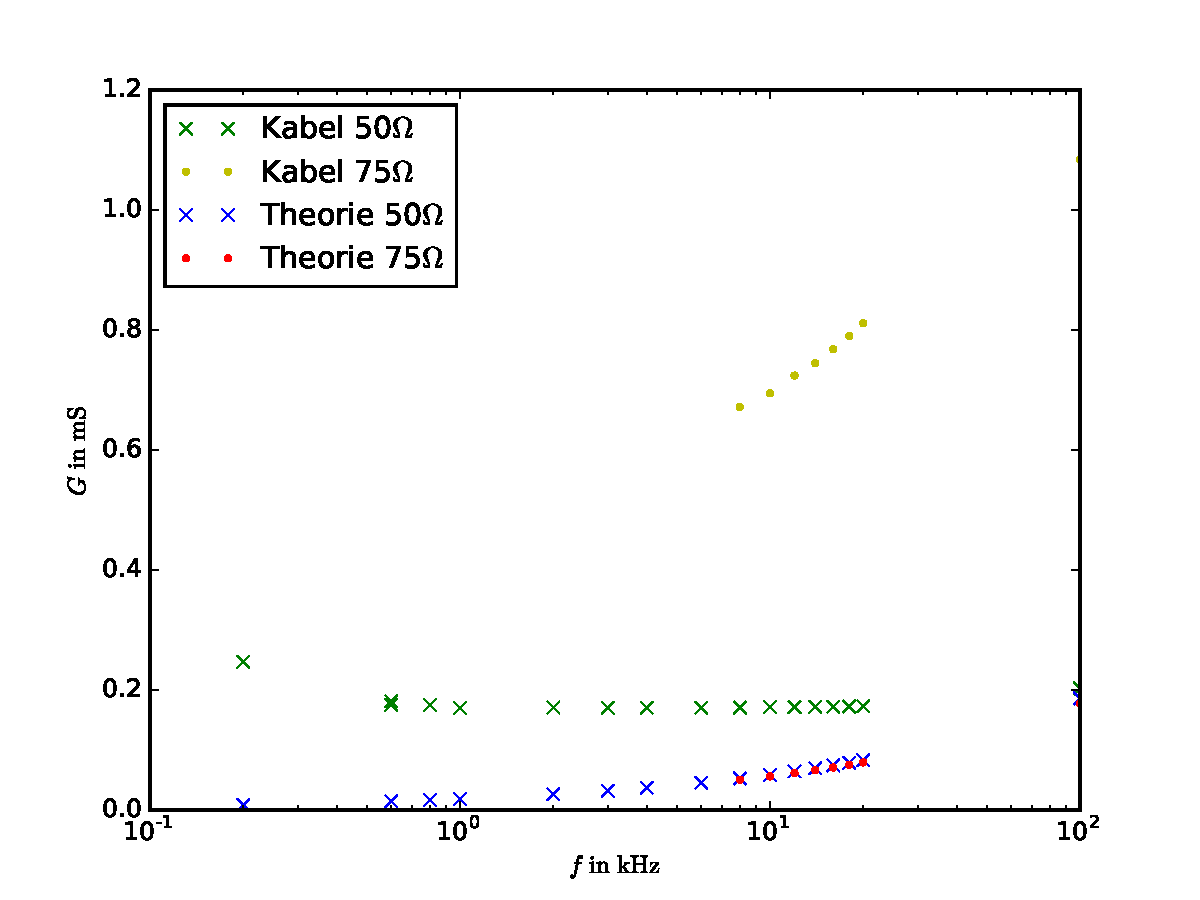
\includegraphics[width=0.8\textwidth]{RLC_DirekteMessung/build/PlotG.pdf}
	\caption{Berechnete Werte für $G$ beim Kurzschluss mit Theoriewert}
	\label{fig:PlotG}
\end{figure}
\begin{align}
	R &= \SI{122.6}{\micro\ohm\per\meter}
 \\
	C &= \SI{105.4}{\pico\farad\per\meter}
 \\
	L &= \SI{237.4}{\nano\farad\per\meter}
 \\
	G &= \SI{54.4}{\nano\siemens\per\meter}

\end{align}